\customsection{Api de animación}
\subsection{Investigación y conceptualización}
Después de imaginar y delimitar  y el problema a tratar, cómo primera instancia, se seleccionó el tipo de entorno de trabajo que sería utilizado para el desarrollo del aplicativo ejecutable de manera local en la vivienda del Solar Decathlon. Durante el transcurso del documento este programa será llamado ``House Manager''.
\vspace{0.5cm}\\
Para seleccionar el entorno de trabajo se realizó una averiguación de los posibles entornos de desarrollo que permitieran implementar programación orientada a objetos en dispositivos embebidos, dentro de los entornos de desarrollo más conocidos se observó: Python, Java, Procesing, C++, entre otros. Todos los anteriores con comunidades muy enfocadas a su mejoramiento constante. Teniendo en cuenta lo anterior realizo un análisis por separado como se puede observar a continuación:
\begin{itemize}
	\item En el caso de C++ se observó que el entorno de trabajo más apropiado para desarrollar aplicativos gráficos era .net, la desventaja de este aplicativo era su estrecha relación con el lenguaje de programación de bajo nivel c\#, por ende el manejo de memoria del programa incrementa en gran medida los costos de desarrollo.
	\item Para Python se observó que los entornos de desarrollo de interfaz gráfica nativos tenían apariencias precarias similar a la nativa de Windows 98, en adición, los frameworks más estéticos tenían un soporte independiente al del lenguaje de programación como tal, por otra parte el lenguaje de programación como tal era multiplataforma y de muy alto nivel, lo que le permitiría al programador desarrollar algoritmos de mayor funcionalidad con menos líneas de código.
	\item En el caso de Java se observó que el entorno de desarrollo para interfaces gráficas era nativo del lenguaje de programación y permitía una mayor flexibilidad a la hora de desarrollar esquemas complejos con la excepción que se debía codificar detalladamente el comportamiento del objeto, lo que significaba más tiempo de trabajo para el programador y archivos con más líneas de código.
\end{itemize}
Como etapa de conceptualización, se realizó una primera versión el diseño del aplicativo principal junto con sus respectivas escenas (Fig \ref{fig_0}). Los elementos utilizados en esta primera etapa de diseño se consistieron principalmente de: botones, caja de opciones, contenedores, y paneles animados. Para esta etapa de conceptualización no se tenía una paleta de colores escogida pero si se buscaba tener en cuenta tonalidades verdes siendo congruentes con la temática amigable con el medio ambiente que rodea al Solar Decathlon, también, se persiguió el poder seleccionar a partir de la pantalla principal diferentes ``sub-aplicativos'' que podrían ser diseñados de manera independiente.

\begin{figure}[htbp]
	\centerline{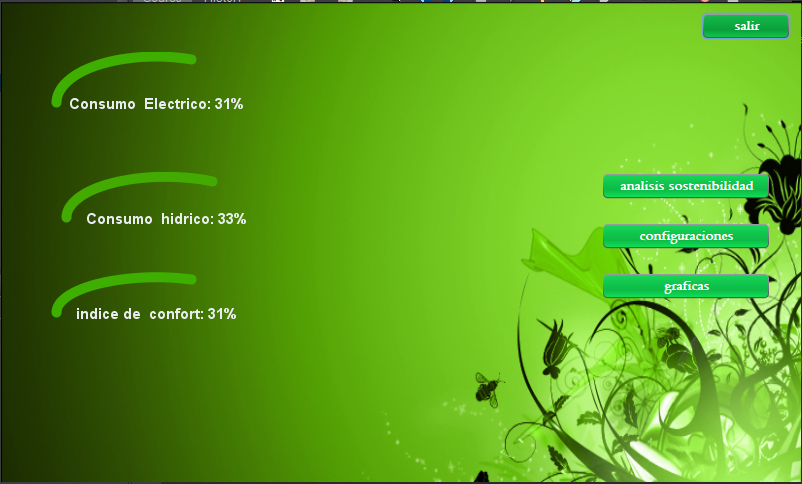
\includegraphics[width=8.5cm]{figuras/houseManager1.png}}
	\caption{Conceptualización inicial del api en sitio. Fuente: propia}
	\label{fig_0}
\end{figure}

Para hacer realidad el diseño de esta primera etapa de conceptualización se utilizó como lenguaje de programación el lenguaje de programación Java puesto que representaba en su mayor parte el lenguaje más utilizado en la Universidad del Valle durante el momento.

\begin{figure}[htbp]
	\centerline{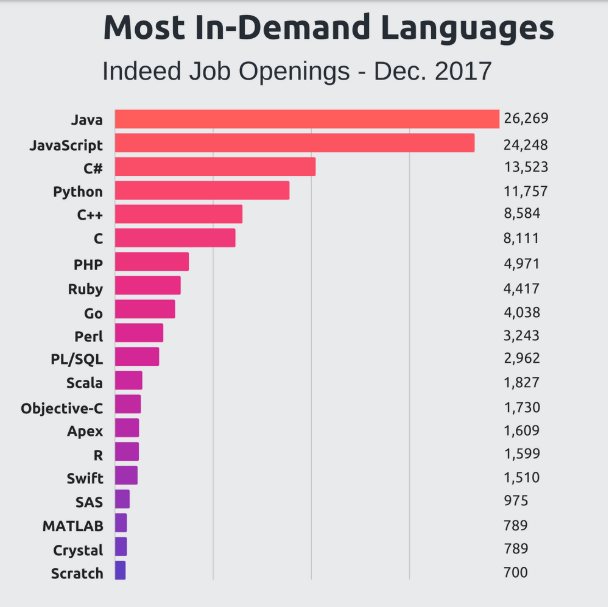
\includegraphics[width=8.5cm]{./figuras/stadistics_job.png}}
	\caption{Estadisticas de los lenguajes de programación con más demanda. Fuente: \cite{stackoverflow2017}}
	\label{fig_1}
\end{figure}

Además, Java es un lenguaje de programación de muy alta demanda, de hecho, el de mayor ofertas de trabajo registradas durante el 2017 en el portal de trabajo internacional \href{https://co.indeed.com/?r=us}{indeed.com}, seguido de JavaScript, c\# y Python, tal como se observa en la figura \ref{fig_1}. Pero esta característica se debe principalmente a que el sistema bancario tradicional esta construido sobre servicios de backend utilizando Java.

\subsection{Api de java}
Todos los objetos implementados para la api fueron desarrollados estrictamente con java puro y sin librerías externas con el objetivo de obtener un código limpio, totalmente multiplataforma y que heredara paquetes únicamente de los módulos \textit{Swing} nativos de java. Como primera instancia se desarrolló el componente funcional de la API, es decir la parte programática, y finalmente se escribió el Javadoc, el cual es un documento integrado que describe como se deben usar los objetos 
\vspace{0.5cm}\\
Normalmente para java es necesario construir y empaquetar el código que contenga la interacción de manera manual con java puro. Por ejemplo, en JavaScript es posible enlazar funciones directamente sin acceder a paquetes adicionales como los ``event listeners'' de java, puesto que todo es considerado un objeto; desde un numero hasta una función.	
\vspace{0.5cm}\\
El primer objeto desarrollado en la Api de java fue el botón personalizado, usando este objeto contenido en la api se puede crear un botón de cualquier tamaño con una, dos o tres imágenes para los estados; ``normal'', ``presionado'' y ``encima''. Un ejemplo de la utilización de la api se puede ver en la figura \ref{fig_2}. Este objeto funciona ajustando automáticamente su tamaño basado en la resolución de las imágenes, esto para complementar con una metodología de diseño: primero el dibujo, luego el programa.

\begin{figure}[htbp]
	\centerline{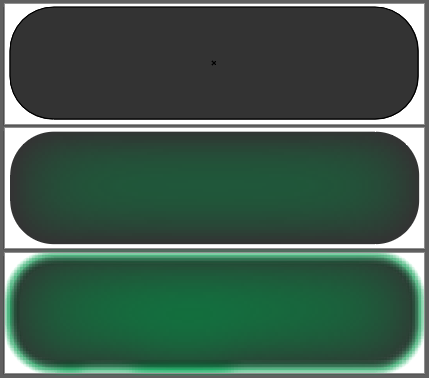
\includegraphics[width=8.5cm]{./figuras/boton.png}}
	\caption{El diseño de estados del botón interactivo. Fuente: propia}
	\label{fig_2}
\end{figure}

El segundo objeto gráfico desarrollado fue un botón expandible o ``caja de opciones'', que permitiera generar un botón desplegable con la posibilidad de modificar texto de manera superficial basado en dos o tres imágenes para la parte superior, inferior y media respectivamente. Un implementación utilizada en la aplicación se puede observar en la figura \ref{fig_3}. Cada una de las imágenes del botón desplegable debe tener sus 3 imágenes de estado: normal, presionado y encima para interactuar de manera dinámica con el mouse.

\begin{figure}[htbp]
	\centerline{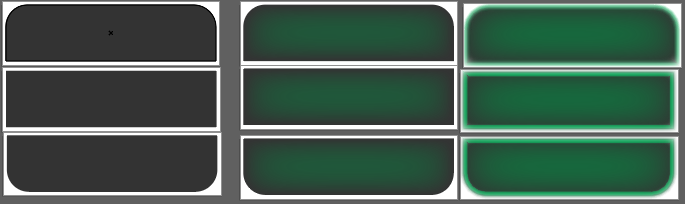
\includegraphics[width=7.5cm]{./figuras/boton_desplegable.png}}
	\caption{El diseño de los estados del botón interactivo desplegable. Fuente: propia}
	\label{fig_3}
\end{figure}

Como tercer objeto gráfico, se desarrolló un objeto de animación que podía mover un objeto tipo swing (esta es la clase madre de la mayoría de los objetos gráficos en java) en 4 posibles direcciones; las dos horizontales y las dos verticales, tal como se observa en la figura \ref{fig_4}. La función permite modificar la ubicación actual del objeto moviéndolo de manera linear con una rata de refresco dada (actualización visual) y una velocidad constante, desde una coordenada X o Y dependiendo de en cual eje coordenado se desee mover el componente.

\begin{figure}[htbp]
	\centerline{
\includegraphics[width=7.5cm]{./figuras/boton_movimiento.png}}
	\caption{Movimiento según la ubicación de la función horizontal. Fuente: propia}
	\label{fig_4}
\end{figure}

El desarrollo de la api fue de importancia para la construcción de la primera versión del aplicativo en sitio, la primera versión se puede observar en la figura \ref{fig_5}, debido a la recursiva implementación gráfica se obtuvo un programa que sobrecargaba un sistema de cómputo completo (portátil Dell con procesador i5 segunda generación, 4gb de ram DDR3, y un disco duro HDD). Por lo tanto se buscó cambiar el entorno de desarrollo a uno con más flexibilidad a la hora del diseño gráfico, con capacidad de funcionar en sistemas de más bajo cómputo tipo Single Computer Boards como la Raspberry o la Beaglebone. Para probar el desempeño de la api, se realizaron pruebas con los elementos ya diseñados en la api de Java y se observó que resultaba una carga para el cpu realizar las animaciones, principalmente, cuando se deseaba mover más de 5 objetos tipo JavaSwing (los objetos gráficos nativos de java).

\begin{figure}[htbp]
	\centerline{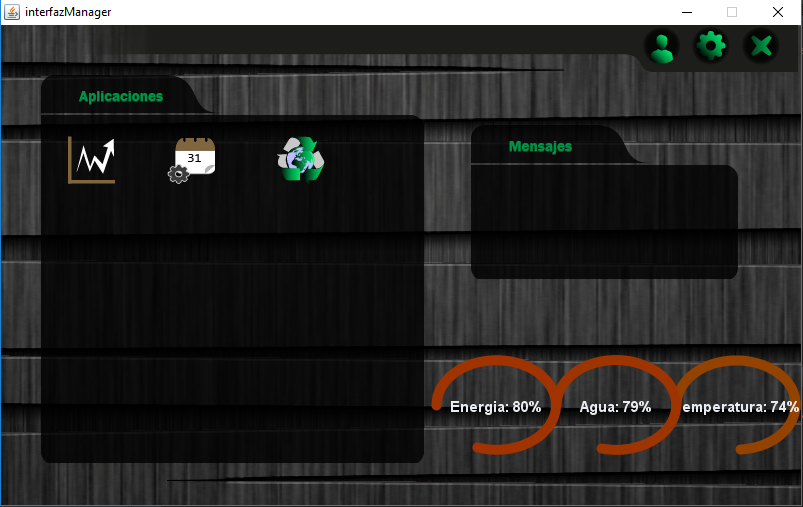
\includegraphics[width=8.5cm]{./figuras/houseManager23.png}}
	\caption{Primer Aproximación del diseño de la interfaz en sitio. Fuente: propia}
	\label{fig_5}
\end{figure}

Después de haber programado los elementos necesarios para generar la estructura básica del aplicativo se replanteo el diseño con una estructura más moderna y parecidas a las tendencias en diseño móvil tal como se observa en la figura \ref{fig_21}, con el objetivo de que se percibiera que ambos aplicativos desarrollados en este sistema podían ofrecer los mismos servicios. Además, generar una experiencia de usuario similar en ambas plataformas

\begin{figure}[htbp]
	\centerline{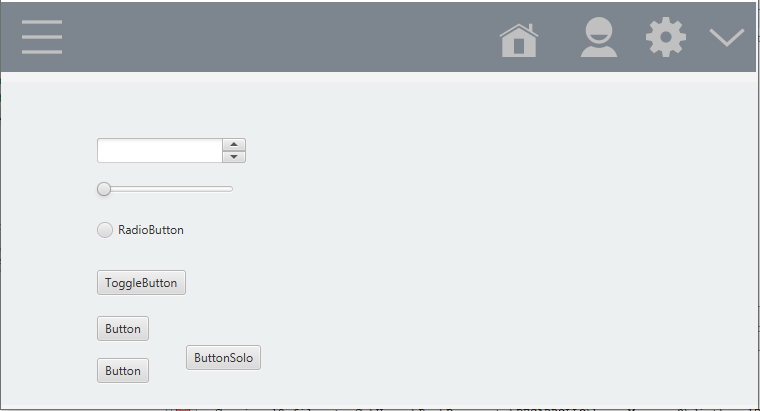
\includegraphics[width=8.5cm]{./figuras/house_manager_version_2.png}}
	\caption{Ajuste de diseño de la interfaz en sitio. Fuente: propia}
	\label{fig_21}
\end{figure}

En un tercer nivel de conceptualización se re diseño la interfaz gráfica estandarizando y simplificando los componentes que esta contenía; se seleccionó la paleta de colores y agregaron algunos nuevos objetos al diseño generalizado como se puede observar en la figura véase en la figura \ref{fig_22}. Para la correcta selección de la paleta de colores se buscó generar una simetría triangular en el espacio de colores HSV, usando como referencia un color sacado del logo oficial de la ``Chameleon House'' (nombre oficial de la casa diseñada para el Solar Decathlon). 

\begin{figure}[htbp]
	\centerline{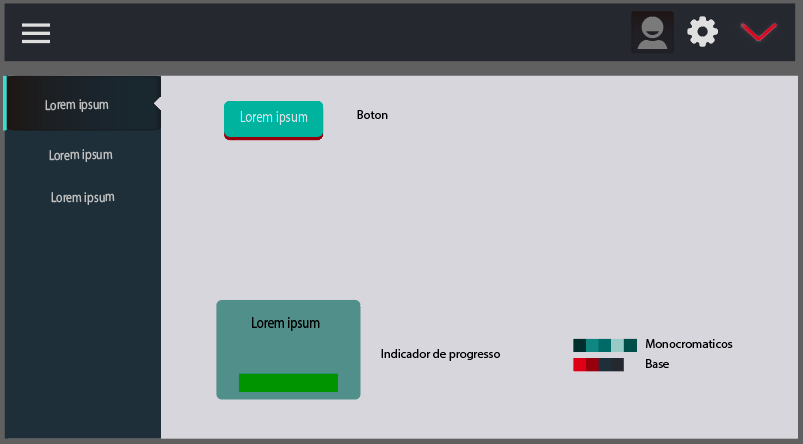
\includegraphics[width=8.5cm]{./figuras/house_manager_version_3.png}}
	\caption{Versión final del concepto de diseño gráfico. Fuente: propia}
	\label{fig_22}
\end{figure}

Debido a la estructura de Java, codificar todos los nuevos objetos resultaba una tarea de mayor trabajo y con baja recompensa, es decir, más líneas de código por objeto. Como solución, se tradujo lo que se tenía desarrollado hasta el momento, a un lenguaje de programación de más alto nivel (Python) y se utilizó un framework exclusivamente para el desarrollo de la interfaz gráfica. Debido a que el framework se trataba de un módulo completamente escrito en C, le permitía a la aplicación tener un mejor rendimiento gráfico.
\vspace{0.5cm}\\
En adición, se cambió el lenguaje de programación para optimizar el tiempo de desarrollo de la aplicación. Teniendo en cuenta que python es un lenguaje de mas alto nivel se decidio cambiar de lenguaje para optimizar el tiempo desarrollo de la aplicacion en sitio. Para ilustrar lo anterior se puede observar un snippet\footnote{En programación un ``snippet'' es un termino para definir una pequeña porción de codigo reusable. Usualmente son unidades operativas que son incorporadas en modulos de programa mas grandes.} de ejemplo para java y python respectivamente:

\begin{Verbatim}[tabsize=4]

public static void POSTRequest() throws IOException {
	final String POST_PARAMS = "";
	System.out.println(POST_PARAMS);
	URL obj = new URL("https://jsonplaceholder.typicode.com/posts");
	HttpURLConnection postConnection = (HttpURLConnection) obj.openConnection();
	postConnection.setRequestMethod("POST");
	postConnection.setRequestProperty("userId", "a1bcdefgh");
	postConnection.setRequestProperty("Content-Type", "application/json");
	postConnection.setDoOutput(true);
	OutputStream os = postConnection.getOutputStream();
	os.write(POST_PARAMS.getBytes());
	os.flush();
	os.close();
	int responseCode = postConnection.getResponseCode();
	System.out.println("POST Response Code :  " + responseCode);
	System.out.println("POST Response Message : " + postConnection.getResponseMessage());
	if (responseCode == HttpURLConnection.HTTP_CREATED) { //success
		BufferedReader in = new BufferedReader(new InputStreamReader(
		postConnection.getInputStream()));
		String inputLine;
		StringBuffer response = new StringBuffer();
		while ((inputLine = in .readLine()) != null) {
			response.append(inputLine);
		} in .close();
		// print result
		System.out.println(response.toString());
	}
}
\end{Verbatim}
El ``snippet'' anterior es utilizado para realizar una solicitud Https tipo post y utiliza 28 lineas de código. Por el contrario, en Python la misma solicitud se puede realizar en 4 lineas de código, como se observa a continuación:

\begin{Verbatim}[tabsize=4]
response = req.post('https://jsonplaceholder.typicode.com/posts', data = None, json = dictionaryObject) 
if response != None:
	print(response.json())      
\end{Verbatim}

Una ventaja de utilizar java como lenguaje de programación es que garantiza de manera efectiva la estructura de los datos durante la ejecución, pero sacrifica tiempo de desarrollo. El anterior ejemplo fue utilizado debido a que la solicitud Https tipo Post es utilizada por los programas cliente del proyecto. Teniendo en cuenta lo anterior, se decidió cambiar el lenguaje de desarrollo a Python inclusive con la Api de desarrollo gráfico terminada.

\subsection{Api de Python y Qt}

El framework utilizado para desarrollar los módulos gráficos se llama Qt y para poder utilizarlo es necesario instalar unas dependencias C específicas y la librería respectiva para Python. Una vez Qt está correctamente configurado el diseño estatico del aplicativo se realiza a partir de un ``lenguaje de marcado'' (markup language) auto generado llamado Qml que define las propiedades gráficas estáticas de los objetos a utilizar, el Qml viene de la mano con un lenguaje tipo ``hoja de estilo'' (style sheet) llamado Qss, a partir del cual se le adjudican propiedades interactivas y estilos que en conjunto son comprendidos por Python y su librería Pyside. El anterior entorno de desarrollo, facilito la implementación de la api puesto que se relacionaba directamente con la forma como se desarrolla frontend para la web.
Para esta etapa de diseño se utilizó una paleta de colores complementarios para los objetos importantes y tonalidades oscuras de grises azulados para los fondos. Todos dentro del espectro de colores de la marca de la casa del Solar Decathlon Latinoamerica de la Universidad del Valle.
\vspace{0.5cm}\\
Teniendo en cuenta el nuevo framework se utilizó la herramienta de diseño de Qt desing (oficial del framework) para codificar de manera automática las propiedades estáticas de la interfaz gráfica. También, se codificaron manualmente las propiedades dinámicas en un archivo de Qss que luego fue cargado por la librería Pyside para ser procesado como un objeto Python. 
\vspace{0.5cm}\\
Primero, se codificó un botón de la misma manera como se implemento el código de la API para Java; con este objeto de Python se logro crear un botón de cualquier tamaño con una, dos o tres imágenes para los estados; ``normal'', ``presionado'' y ``encima''. Un ejemplo de la utilización de la api se puede ver en la figura \ref{fig_19}.
\vspace{0.5cm}\\
\begin{figure}[htbp]
	\centerline{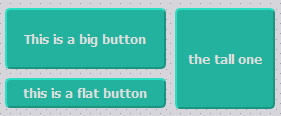
\includegraphics[width=7.5cm]{./figuras/qt_button.png}}
	\caption{Botón de tamaño flexible genérico de la api de qt. Fuente: propia}
	\label{fig_19}
\end{figure}

Segundo se codificó un botón genérico con las mismas funcionalidades del botón anterior, pero en lugar de funcionar basado en imágenes funcionaba con un color dado y las interacciones ``normal'', ``presionado'' y ``encima'' son calculadas atenuando y resaltando el color para generar un efecto de sombra e iluminación. Para el aplicativo se utilizó el color mostrado en la figura \ref{fig_20}.
\vspace{0.5cm}\\
Tercero, se desarrolló un expandible o ``caja de opciones'', personalizada, para ello se modificó el objeto de Qss “QOptionbar” que permite generar un botón desplegable con la posibilidad de modificar texto de manera superficial basado en un color especifico.
\vspace{0.5cm}\\
Cuarto, se programó una barra deslizable para facilitar el proceso de ingresar datos numéricos a la aplicación desde una interfaz táctil. Nuevamente se usaron los colores de la paleta de colores seleccionada y se optó por la solución de diseño más sencilla posible tal como se puede ver en la imagen \ref{fig_20}.

\begin{figure}[htbp]
	\centerline{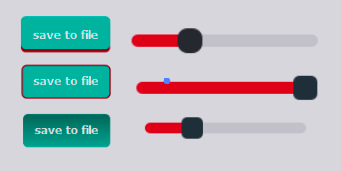
\includegraphics[width=7.5cm]{./figuras/qt_button_slide.png}}
	\caption{Boton de tamaño fijo usando imágenes y slider. Fuente: propia}
	\label{fig_20}
\end{figure}

Finalmente se personalizaron los colores de todos los espacios y elementos secundarios utilizados, como: la gráfica, la barra de menú, los botones especiales del menú, etc. Con un total de 6 elementos diseñados e implementados capaces de re utilizare para otras interfaces.


